%adding correction for percentage of skin
\subsubsection*{Algorithm}
We noticed that in the case where the target image has relatively dark shadows such as in Figure \ref{img:input_hands_1_light}, the average colour calculated for the target hand is too dark, causing the skin colour of the results to appear darker than the skin colour of the target. We correct this by changing the way will calculate the average skin colour of the target hand with only 10\% of the brightest pixel in the skin patch used to calculate the average. As Figure \ref{img:10_perc_mask} shows, the areas with shadows are no longer used for calculating the average colour of the target hand.

% \begin{equation} \label{eq:prop_corr_algo}
%   r'' = \left.
%   \begin{dcases}
%     \displaystyle \mean{r'} - \frac{(\mean{r'} - r')}{\alpha}, & \text{for } r' < \mean{r'} \\
%     \displaystyle r', & \text{for } r' \geq \mean{r'} \\
%   \end{dcases}
%   \right.\\
% \end{equation}

% \nomenclature{$r''$}{Value of the red channel of the pixel after a second algorithm is applied.}
% \nomenclature{$\mean{r'}$}{Average value of the red channel of the hand image outputted by the first algorithm.}

% Where $\alpha$ is a constant, $\alpha  > 1$. The same equation applies for the $g$ and $b$ channels.

% \subsubsection*{Results}
% See Tables in Appendix \ref{app:prop_corr_a1p1}, for the complete results for $\alpha = 1.1$. A portion of the results is reproduced here for convenience.
% \begin{longtable}{|N||c|c|c|}
	\caption{Test results of proportional brightening with correction for dark spots and using brightest 10 percent of pixels to calculate average colour, $\alpha$ = 1.1\label{tab:prop_correct_test_a1p1_ave10}}\\
	\hline
	\multicolumn{1}{|c||}{No.} & Original & Target & Result \\ 
	\hline
	  \ref{row:PY_NAME_hand_dark_to_hand_brown} &
  \begin{minipage}{.29\textwidth}
    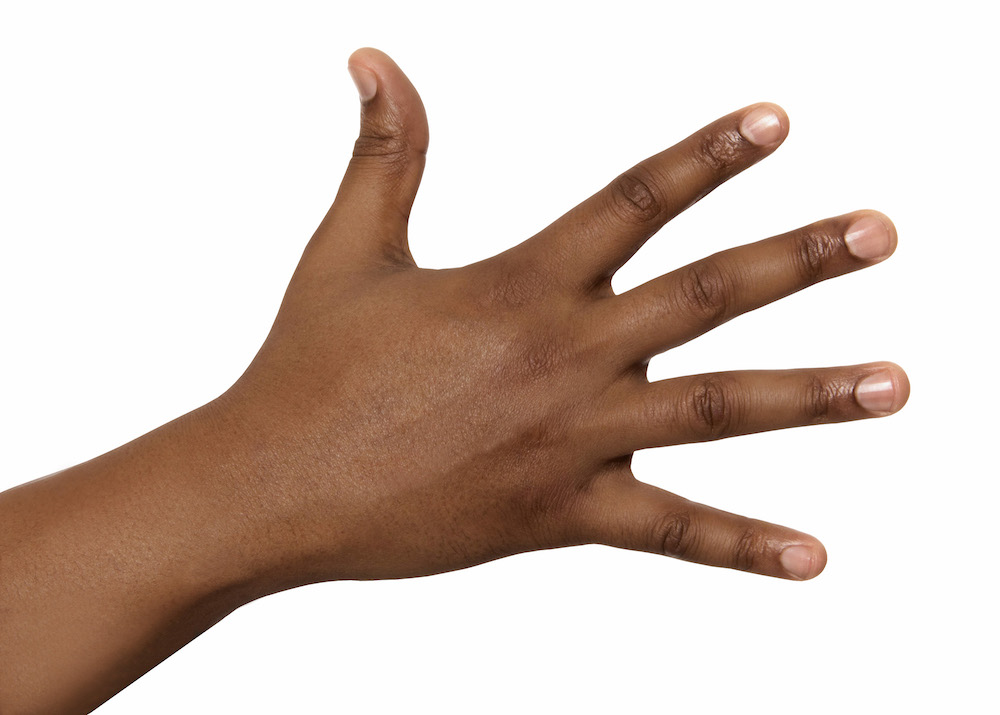
\includegraphics[width=\textwidth,height=\textheight,keepaspectratio]{../inputs/hand_dark.jpg}
  \end{minipage} & 
  \begin{minipage}{.29\textwidth}
    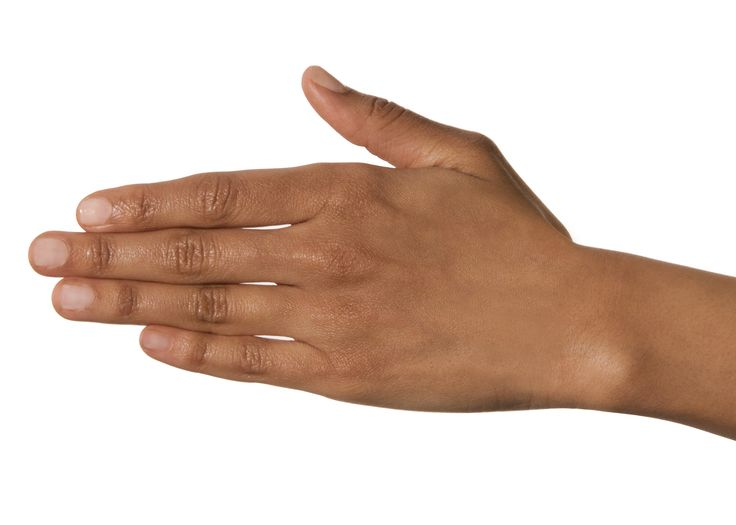
\includegraphics[width=\textwidth,height=\textheight,keepaspectratio]{../inputs/hand_brown.jpg}
  \end{minipage} & 
  \begin{minipage}{.29\textwidth}
    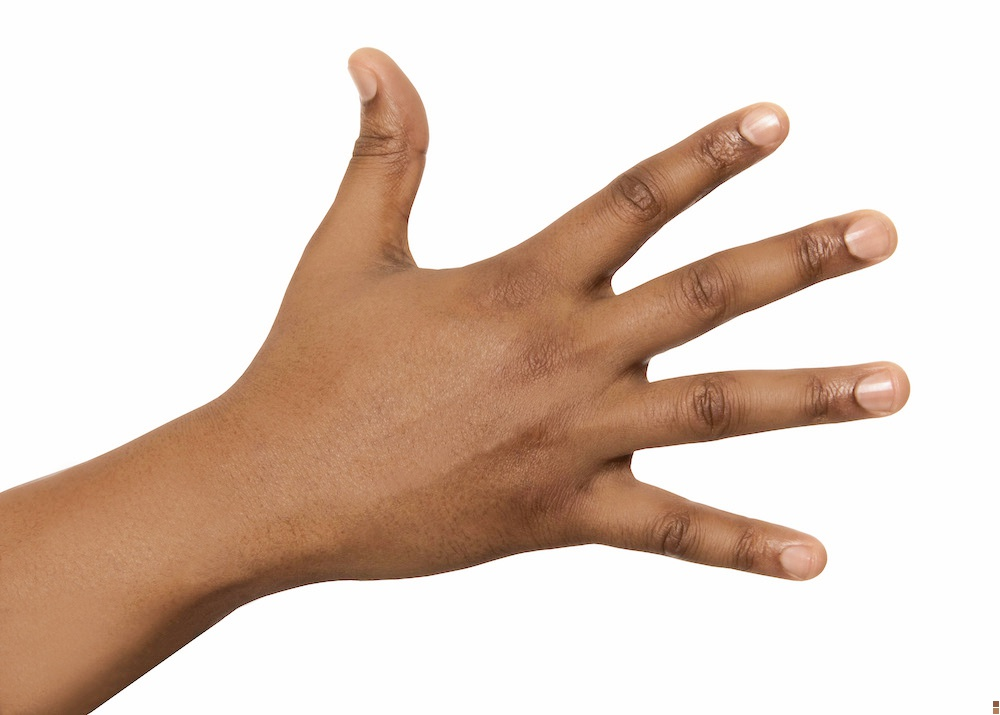
\includegraphics[width=\textwidth,height=\textheight,keepaspectratio]{../rc_test/outputs/20170524_prop_corr_1p1_ave_5/hand_dark_to_hand_brown.jpg}
  \end{minipage} \\
\hline
	  \label{row:PY_NAME_hand_dark_to_hand_light} &
  \begin{minipage}{.29\textwidth}
    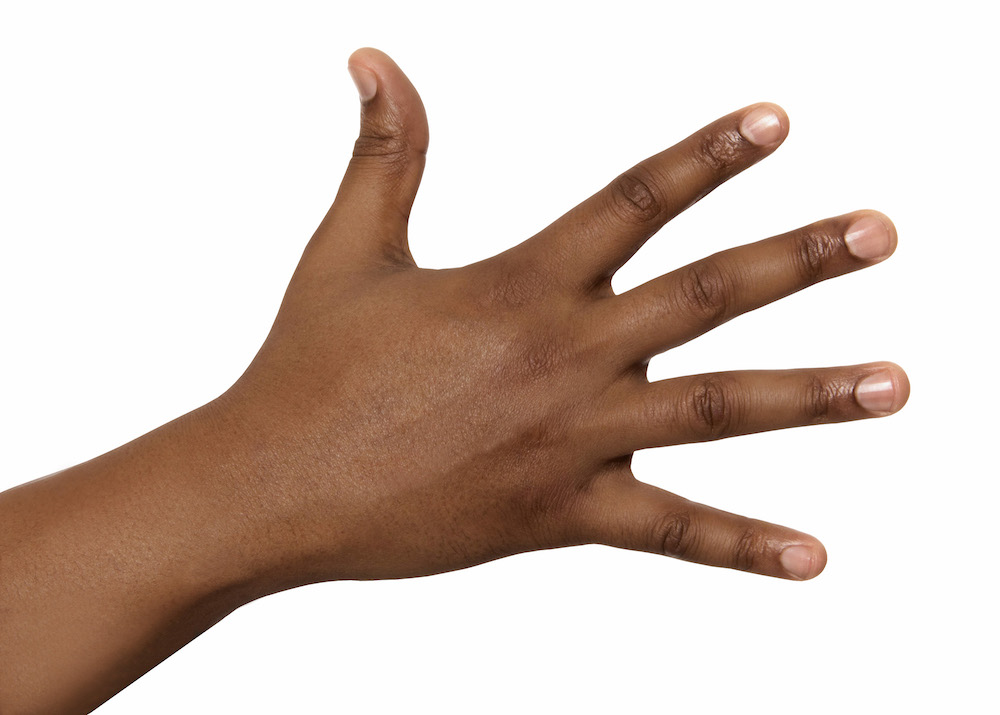
\includegraphics[width=\textwidth,height=\textheight,keepaspectratio]{../inputs/hand_dark.jpg}
  \end{minipage} & 
  \begin{minipage}{.29\textwidth}
    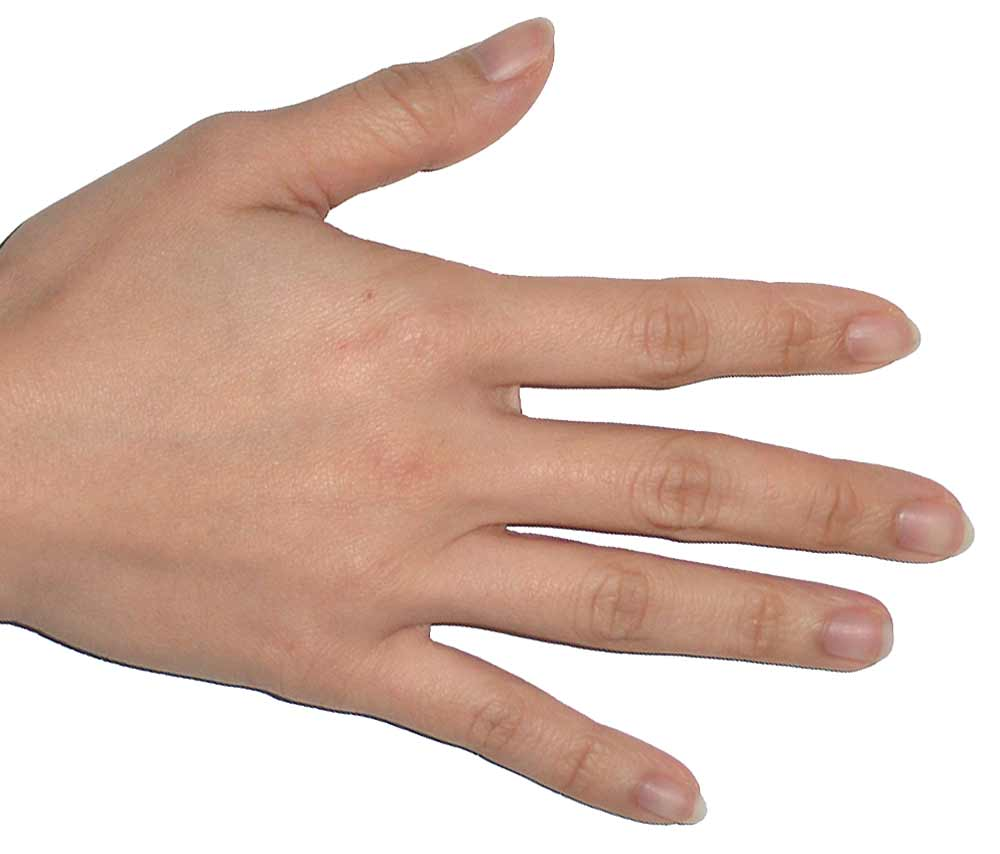
\includegraphics[width=\textwidth,height=\textheight,keepaspectratio]{../inputs/hand_light.jpg}
  \end{minipage} & 
  \begin{minipage}{.29\textwidth}
    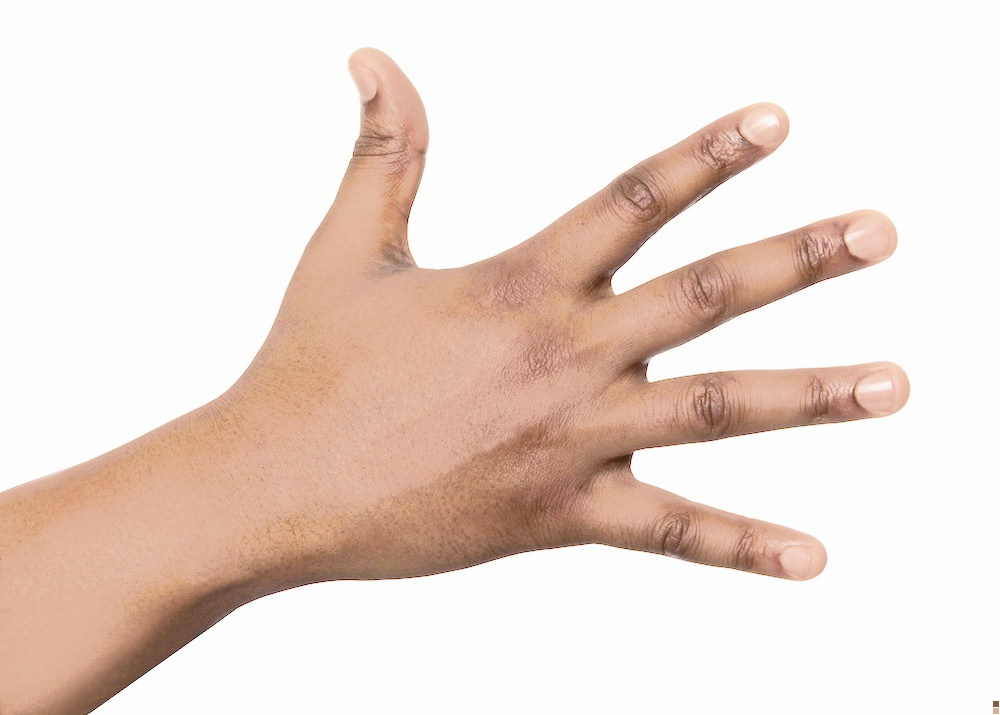
\includegraphics[width=\textwidth,height=\textheight,keepaspectratio]{../rc_test/outputs/20170524_prop_corr_1p1_ave_5/hand_dark_to_hand_light.jpg}
  \end{minipage} \\
\hline
	  \label{row:PY_NAME_hand_dark_to_hand_pale} &
  \begin{minipage}{.29\textwidth}
    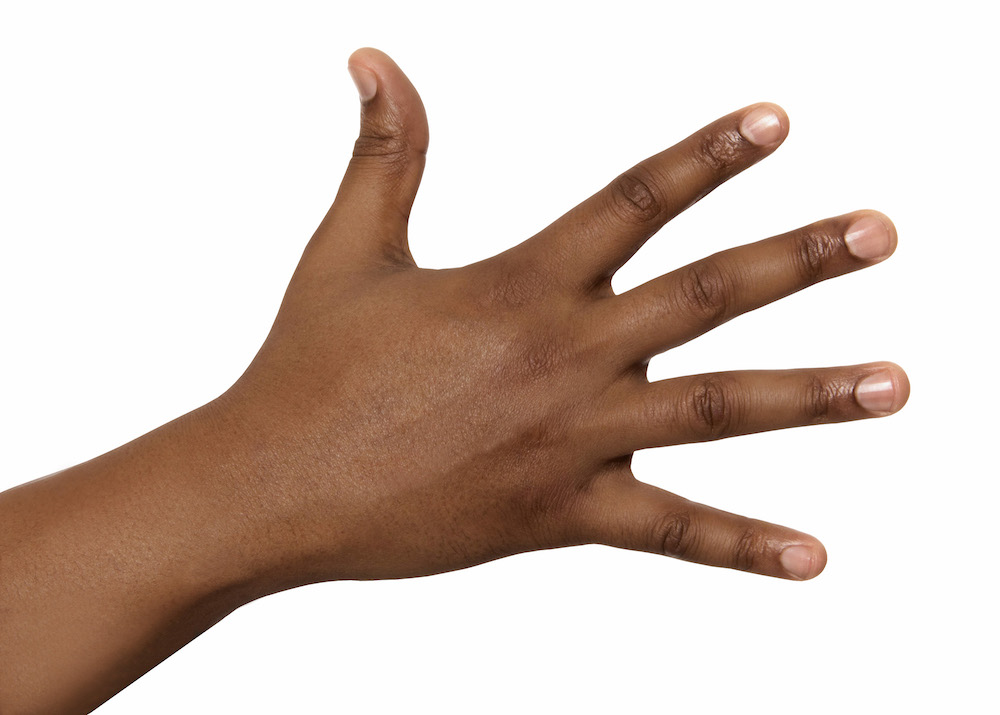
\includegraphics[width=\textwidth,height=\textheight,keepaspectratio]{../inputs/hand_dark.jpg}
  \end{minipage} & 
  \begin{minipage}{.29\textwidth}
    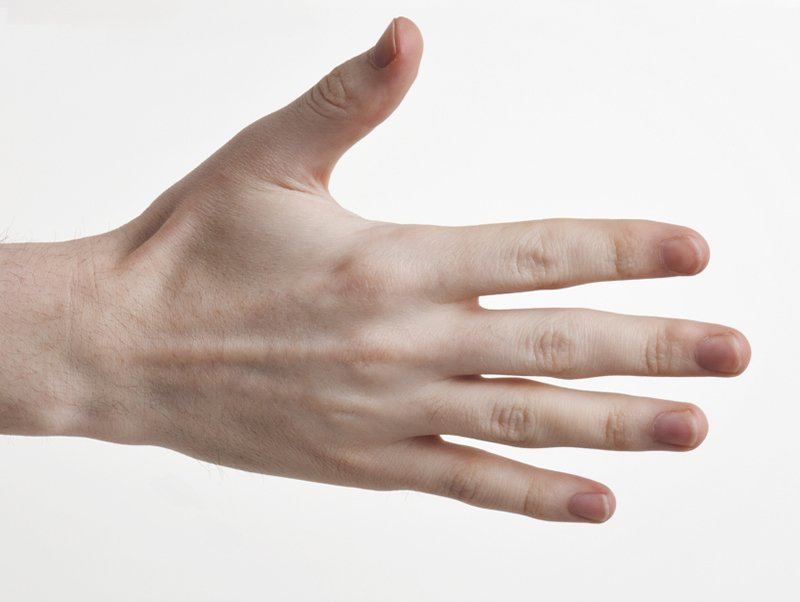
\includegraphics[width=\textwidth,height=\textheight,keepaspectratio]{../inputs/hand_pale.jpg}
  \end{minipage} & 
  \begin{minipage}{.29\textwidth}
    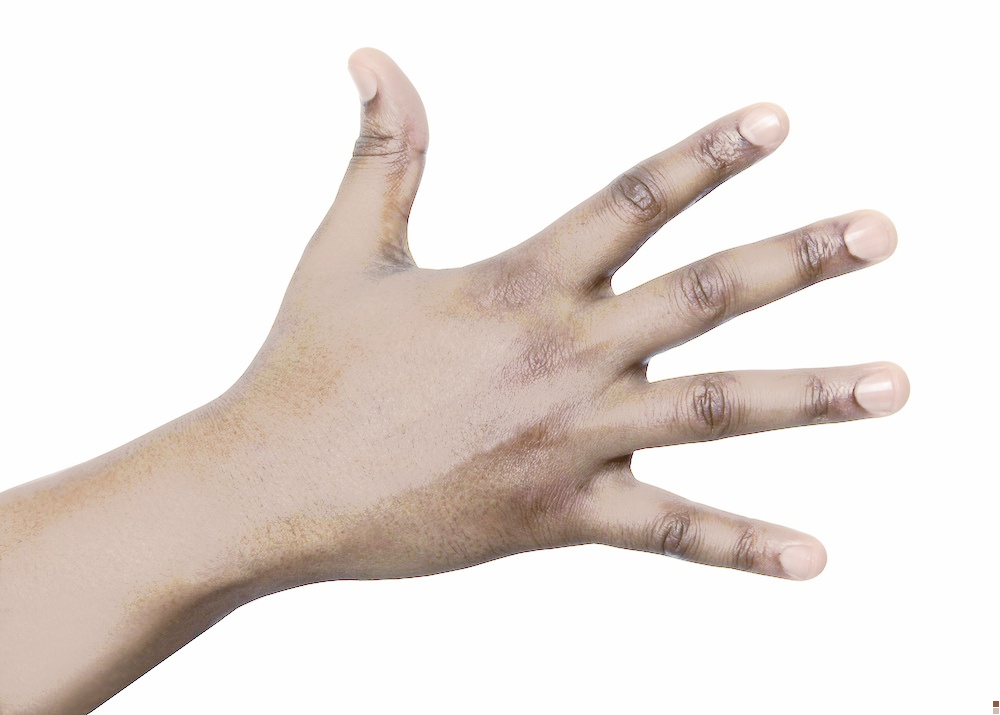
\includegraphics[width=\textwidth,height=\textheight,keepaspectratio]{../rc_test/outputs/20170524_prop_corr_1p1_ave_5/hand_dark_to_hand_pale.jpg}
  \end{minipage} \\
\hline
	  \label{row:PY_NAME_hand_brown_to_hand_dark} &
  \begin{minipage}{.29\textwidth}
    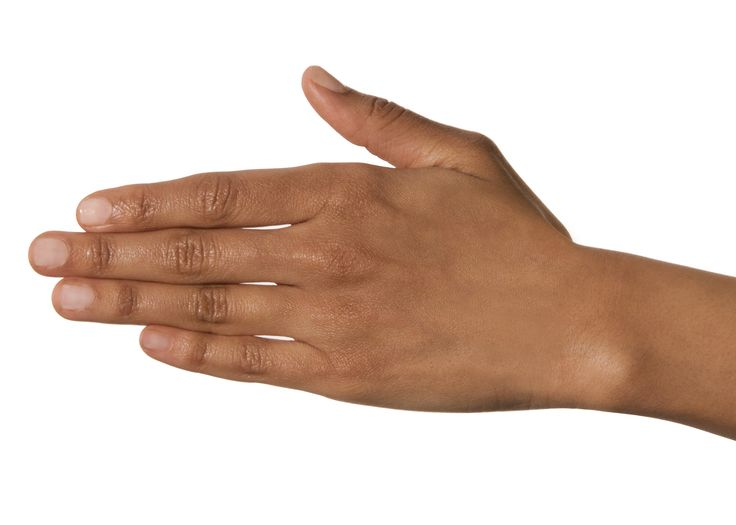
\includegraphics[width=\textwidth,height=\textheight,keepaspectratio]{../inputs/hand_brown.jpg}
  \end{minipage} & 
  \begin{minipage}{.29\textwidth}
    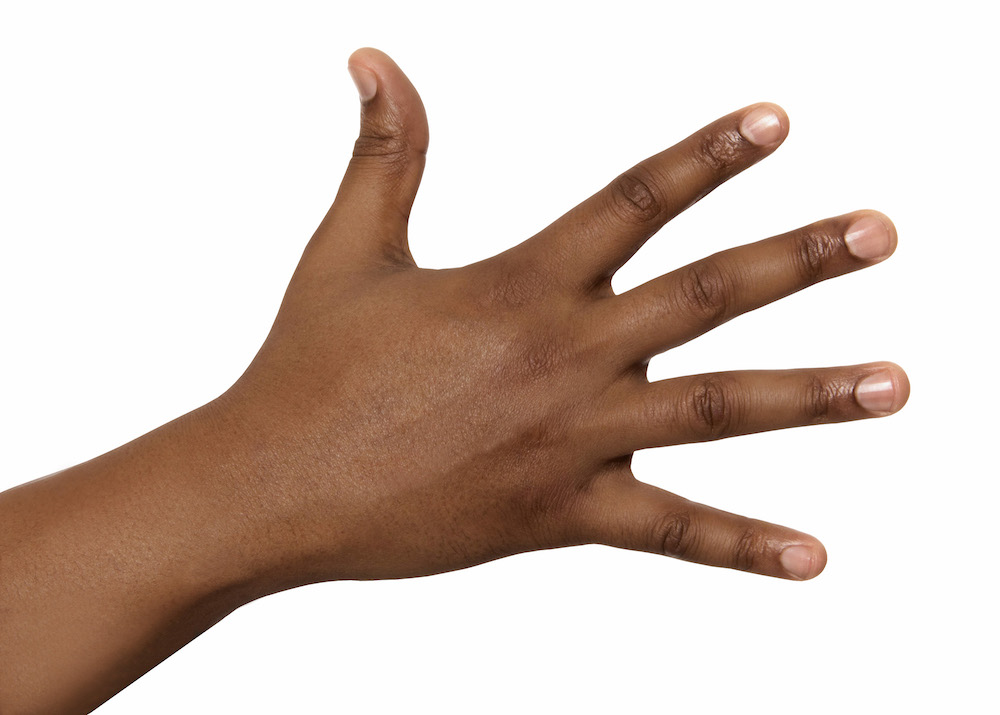
\includegraphics[width=\textwidth,height=\textheight,keepaspectratio]{../inputs/hand_dark.jpg}
  \end{minipage} & 
  \begin{minipage}{.29\textwidth}
    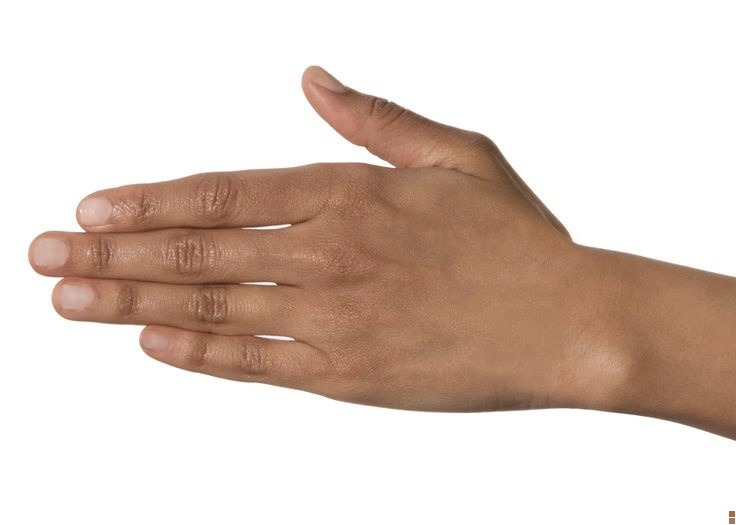
\includegraphics[width=\textwidth,height=\textheight,keepaspectratio]{../rc_test/outputs/20170524_prop_corr_1p1_ave_10/hand_brown_to_hand_dark.jpg}
  \end{minipage} \\
\hline
	  \label{row:PY_NAME_hand_brown_to_hand_light} &
  \begin{minipage}{.29\textwidth}
    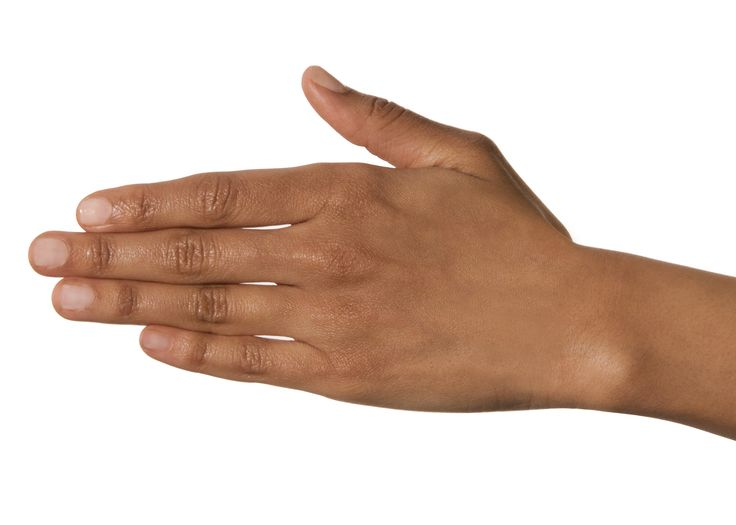
\includegraphics[width=\textwidth,height=\textheight,keepaspectratio]{../inputs/hand_brown.jpg}
  \end{minipage} & 
  \begin{minipage}{.29\textwidth}
    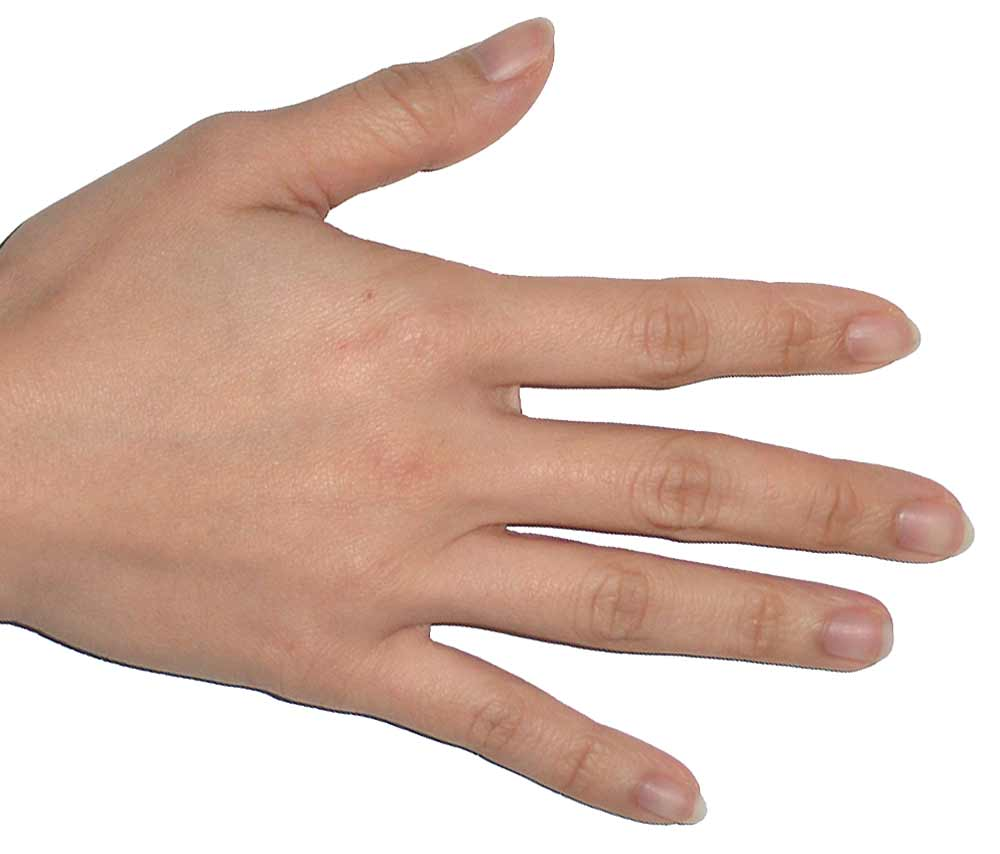
\includegraphics[width=\textwidth,height=\textheight,keepaspectratio]{../inputs/hand_light.jpg}
  \end{minipage} & 
  \begin{minipage}{.29\textwidth}
    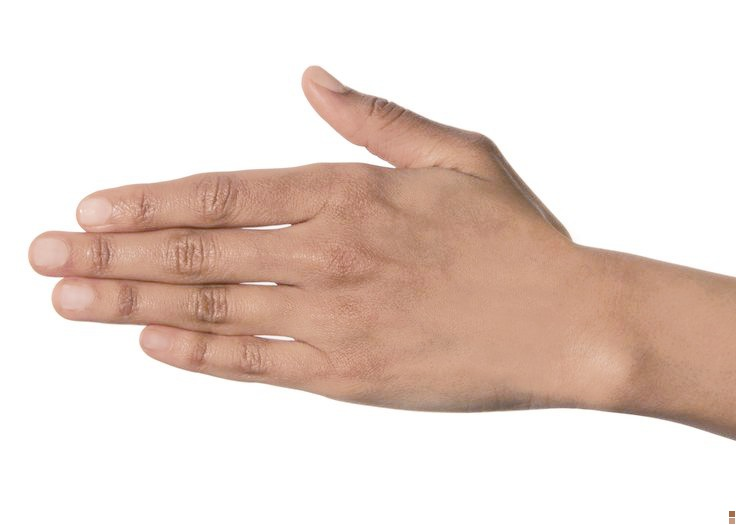
\includegraphics[width=\textwidth,height=\textheight,keepaspectratio]{../rc_test/outputs/20170524_prop_corr_1p1_ave_100/hand_brown_to_hand_light.jpg}
  \end{minipage} \\
\hline
	  \ref{row:PY_NAME_hand_brown_to_hand_pale} &
  \begin{minipage}{.29\textwidth}
    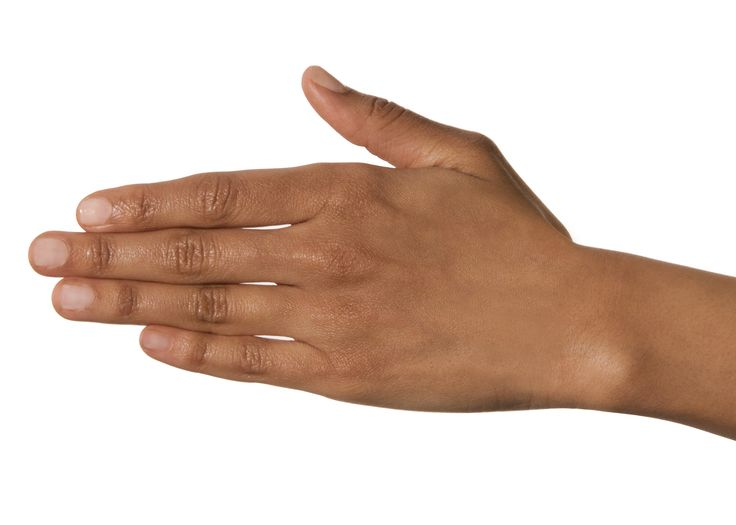
\includegraphics[width=\textwidth,height=\textheight,keepaspectratio]{../inputs/hand_brown.jpg}
  \end{minipage} & 
  \begin{minipage}{.29\textwidth}
    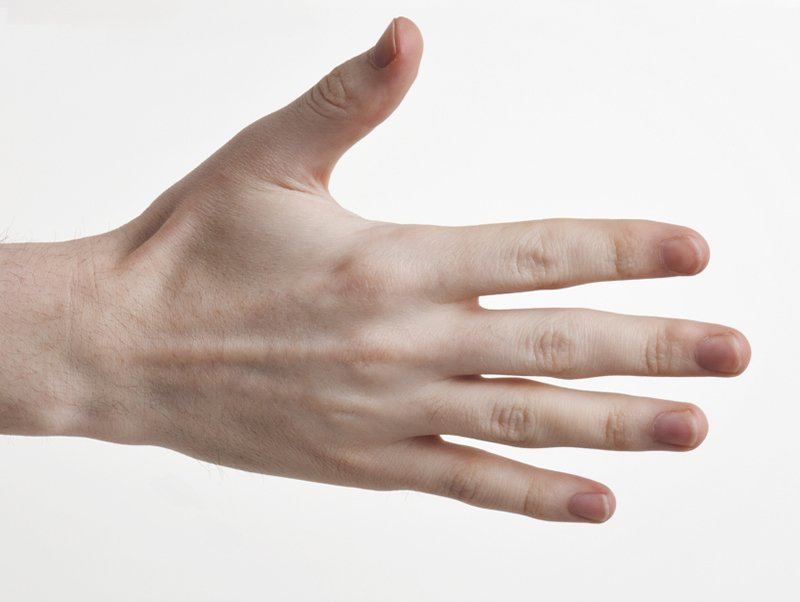
\includegraphics[width=\textwidth,height=\textheight,keepaspectratio]{../inputs/hand_pale.jpg}
  \end{minipage} & 
  \begin{minipage}{.29\textwidth}
    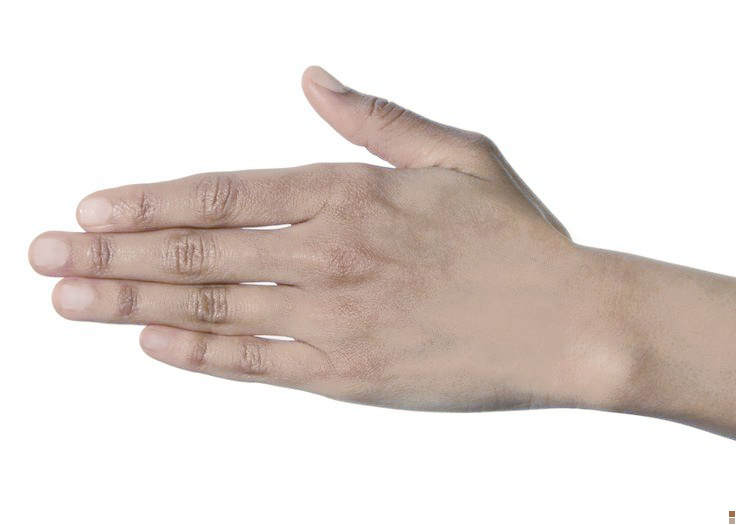
\includegraphics[width=\textwidth,height=\textheight,keepaspectratio]{../rc_test/outputs/20170524_prop_corr_1p1_ave_25/hand_brown_to_hand_pale.jpg}
  \end{minipage} \\
\hline
	  \label{row:PY_NAME_hand_light_to_hand_dark} &
  \begin{minipage}{.29\textwidth}
    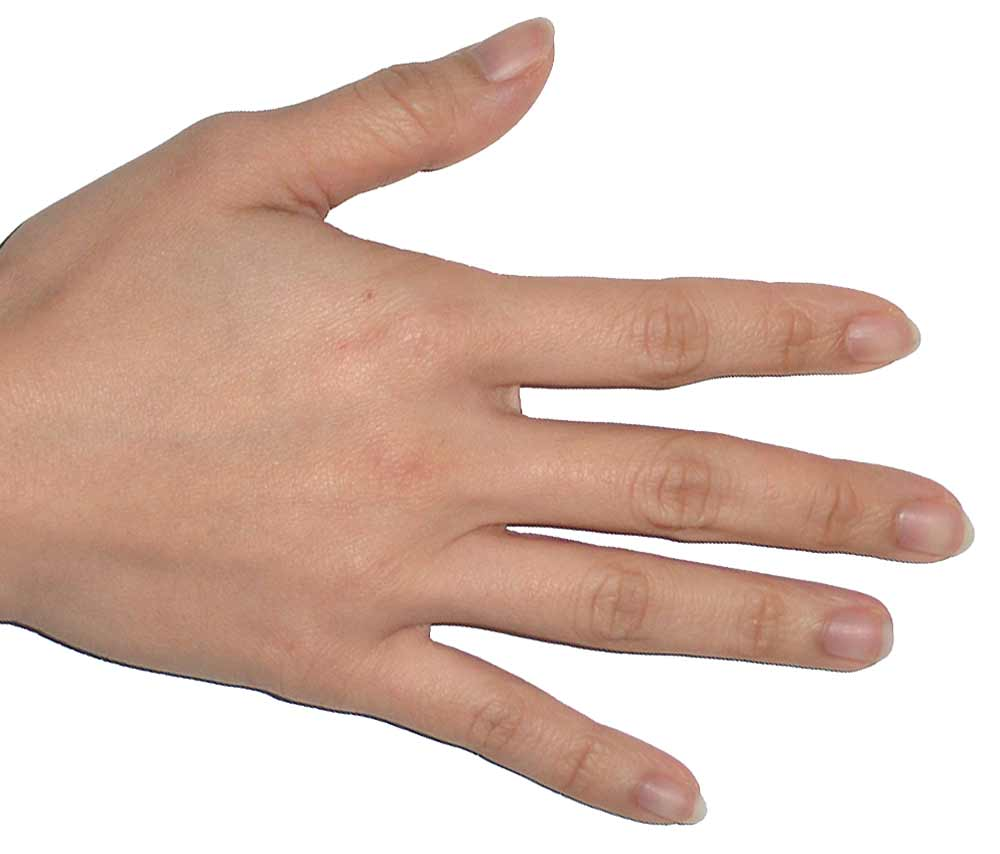
\includegraphics[width=\textwidth,height=\textheight,keepaspectratio]{../inputs/hand_light.jpg}
  \end{minipage} & 
  \begin{minipage}{.29\textwidth}
    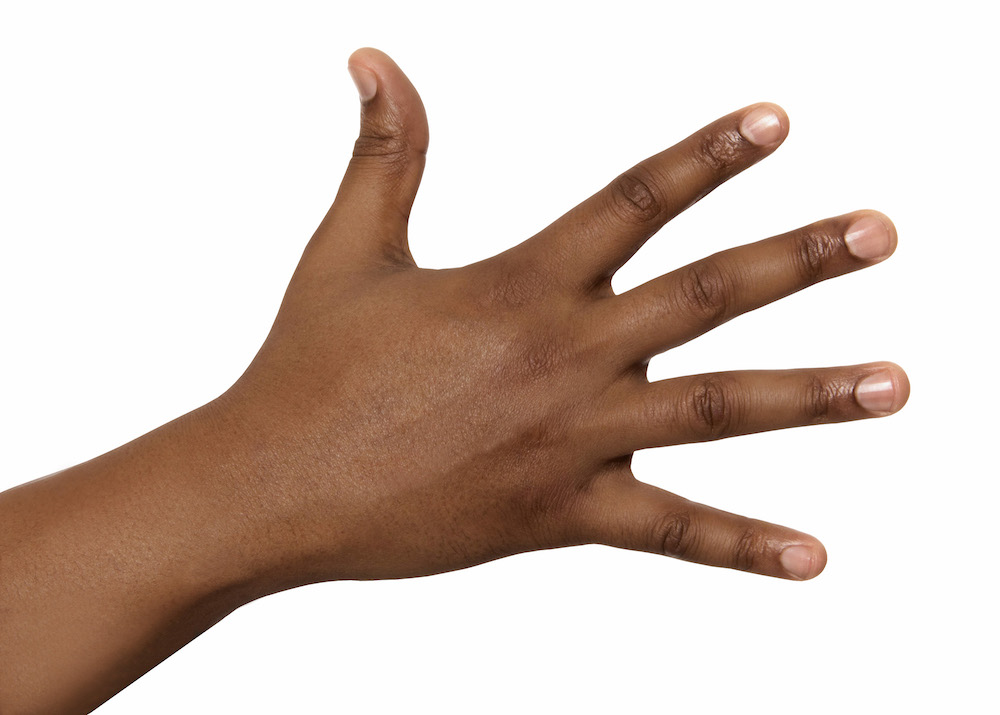
\includegraphics[width=\textwidth,height=\textheight,keepaspectratio]{../inputs/hand_dark.jpg}
  \end{minipage} & 
  \begin{minipage}{.29\textwidth}
    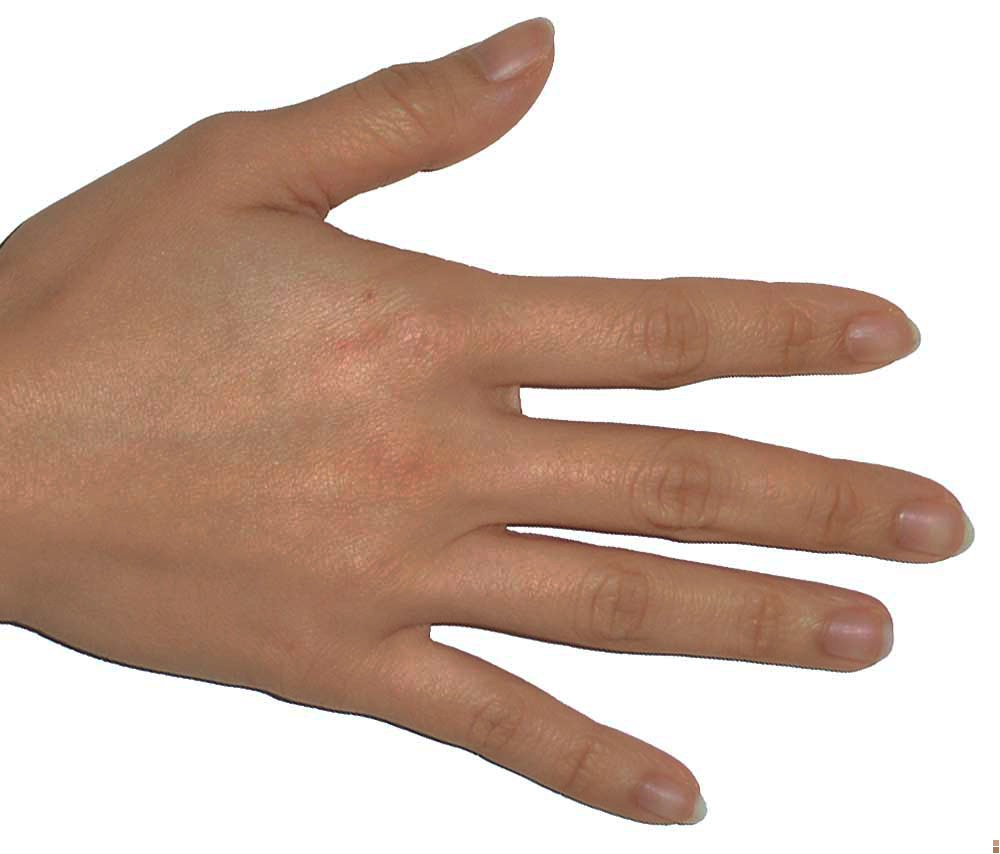
\includegraphics[width=\textwidth,height=\textheight,keepaspectratio]{../rc_test/outputs/20170524_prop_corr_1p1_ave_5/hand_light_to_hand_dark.jpg}
  \end{minipage} \\
\hline
	  \label{row:PY_NAME_hand_light_to_hand_brown} &
  \begin{minipage}{.29\textwidth}
    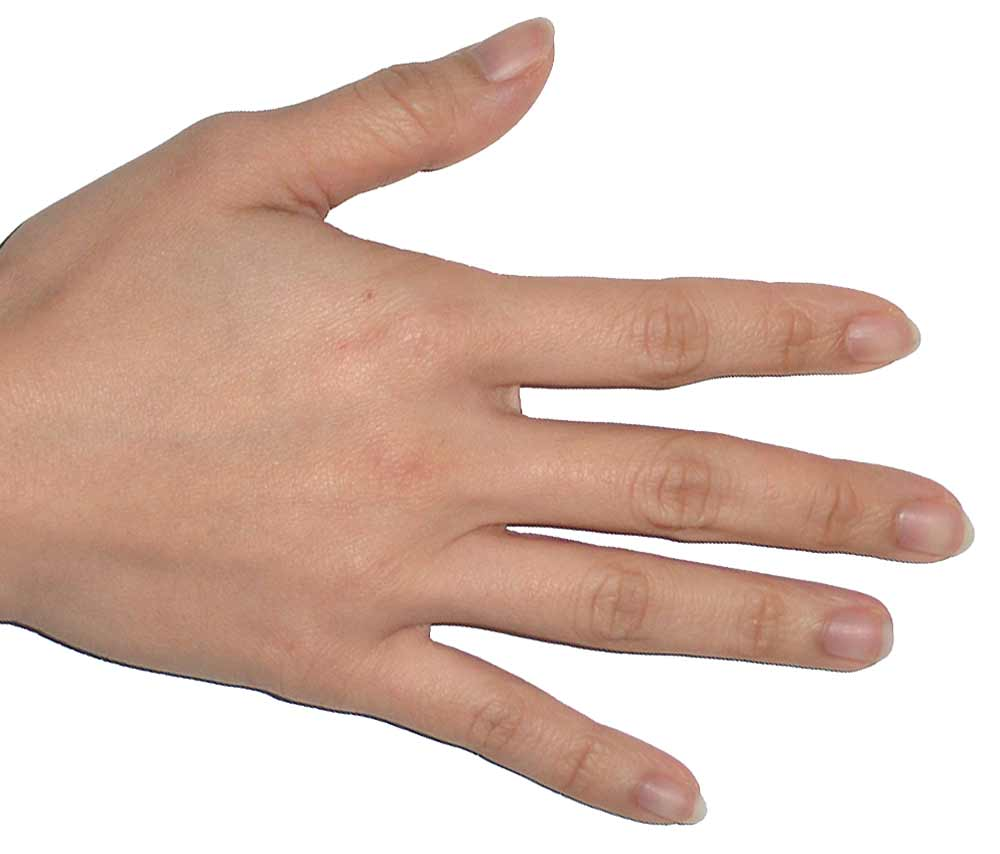
\includegraphics[width=\textwidth,height=\textheight,keepaspectratio]{../inputs/hand_light.jpg}
  \end{minipage} & 
  \begin{minipage}{.29\textwidth}
    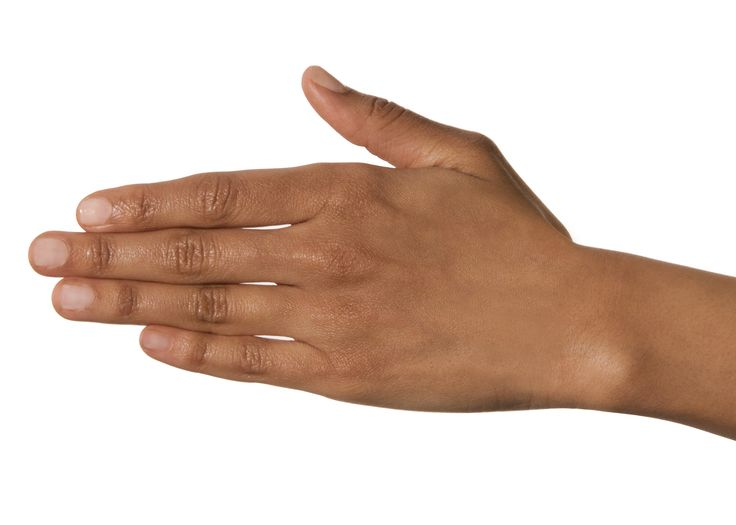
\includegraphics[width=\textwidth,height=\textheight,keepaspectratio]{../inputs/hand_brown.jpg}
  \end{minipage} & 
  \begin{minipage}{.29\textwidth}
    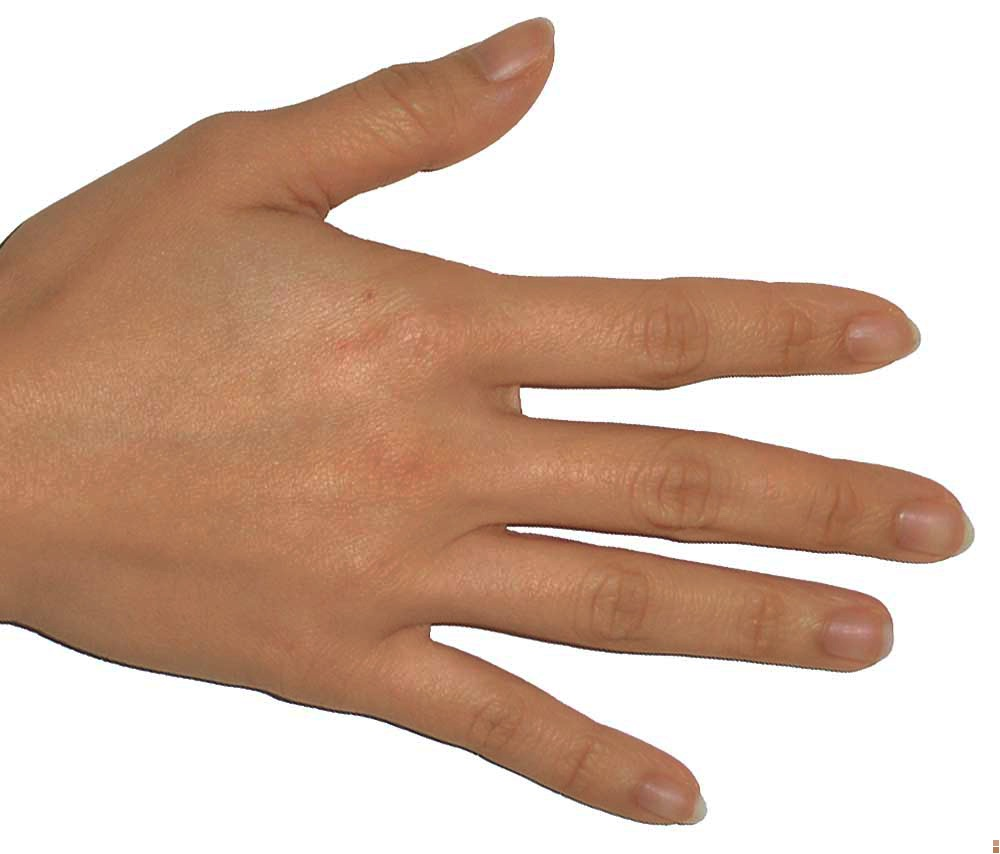
\includegraphics[width=\textwidth,height=\textheight,keepaspectratio]{../rc_test/outputs/20170524_prop_corr_1p1_ave_5/hand_light_to_hand_brown.jpg}
  \end{minipage} \\
\hline
	  \label{row:PY_NAME_hand_light_to_hand_pale} &
  \begin{minipage}{.29\textwidth}
    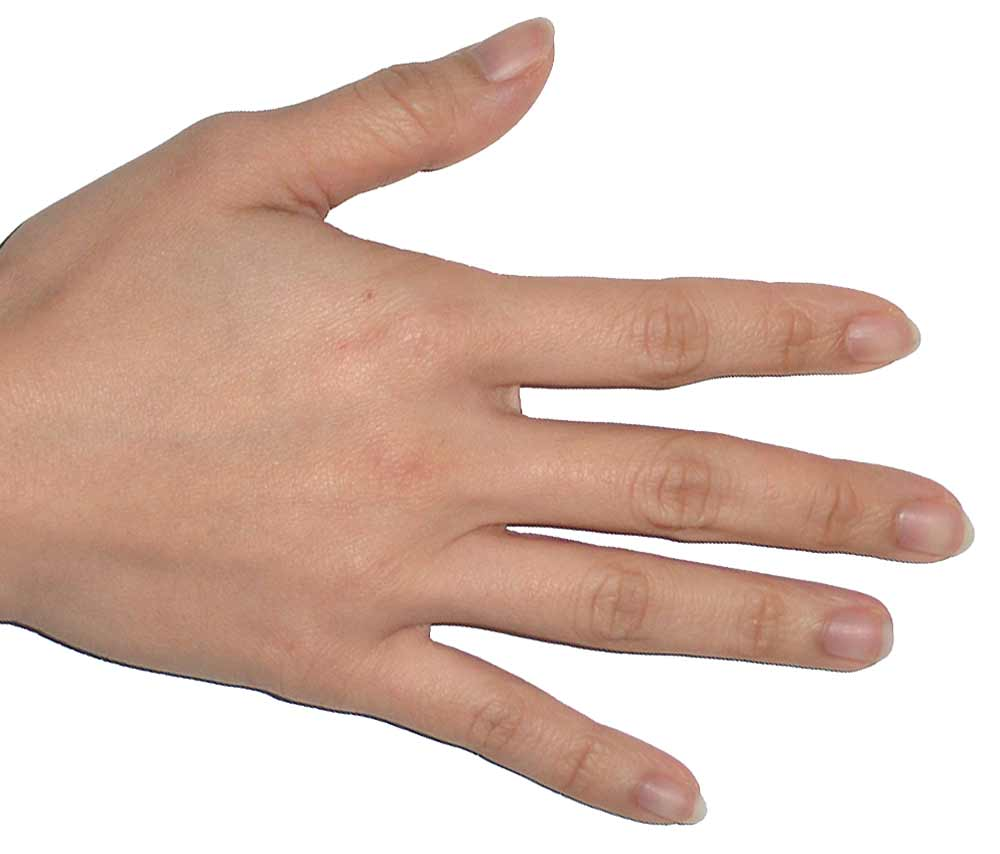
\includegraphics[width=\textwidth,height=\textheight,keepaspectratio]{../inputs/hand_light.jpg}
  \end{minipage} & 
  \begin{minipage}{.29\textwidth}
    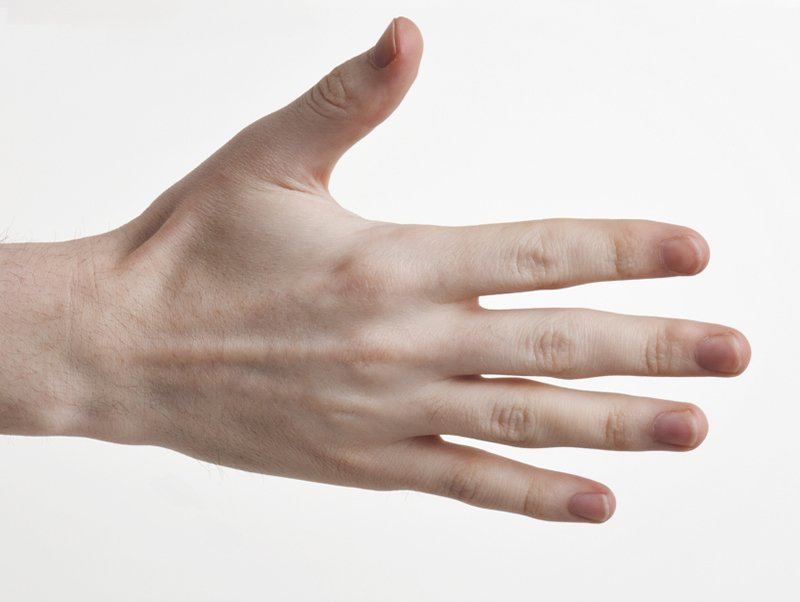
\includegraphics[width=\textwidth,height=\textheight,keepaspectratio]{../inputs/hand_pale.jpg}
  \end{minipage} & 
  \begin{minipage}{.29\textwidth}
    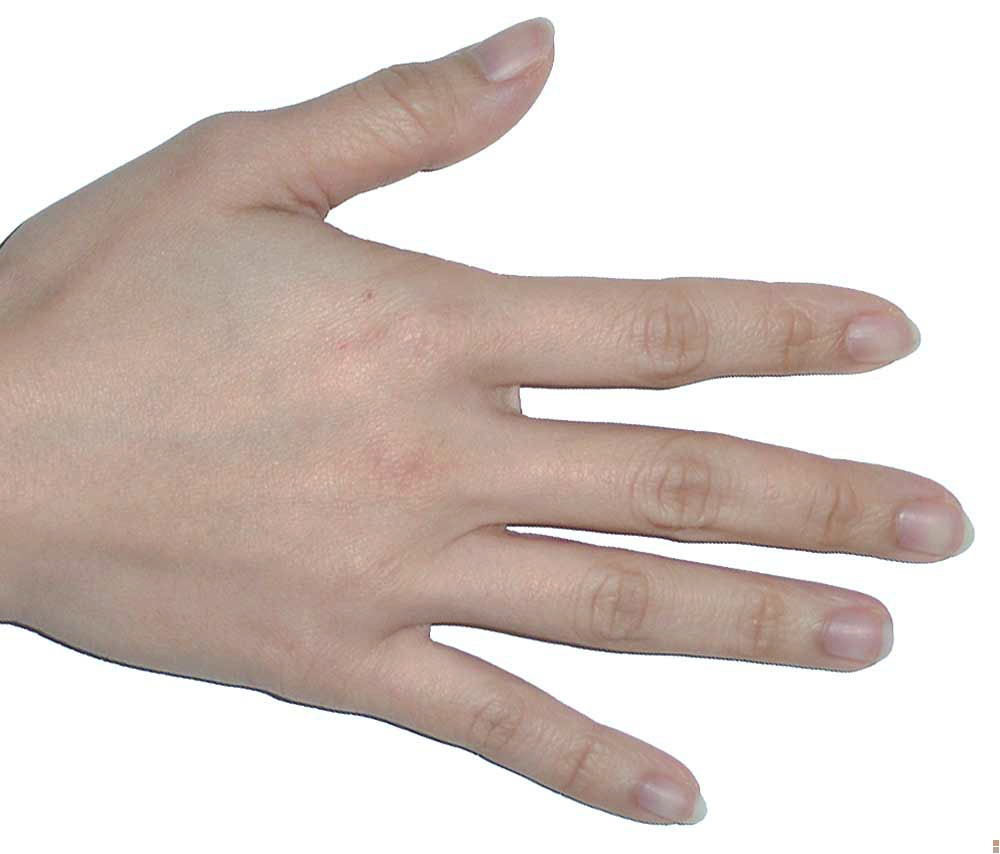
\includegraphics[width=\textwidth,height=\textheight,keepaspectratio]{../rc_test/outputs/20170524_prop_corr_1p1_ave_25/hand_light_to_hand_pale.jpg}
  \end{minipage} \\
\hline
	  \ref{row:PY_NAME_hand_pale_to_hand_dark} &
  \begin{minipage}{.29\textwidth}
    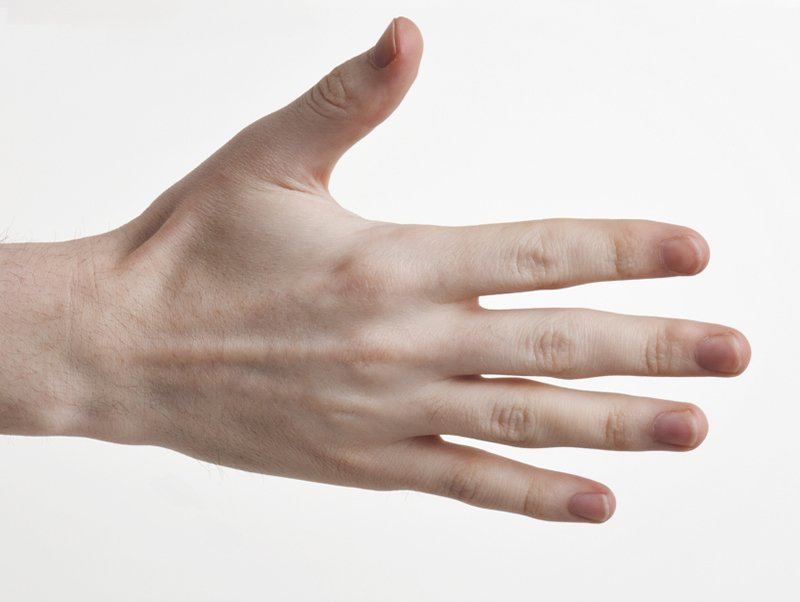
\includegraphics[width=\textwidth,height=\textheight,keepaspectratio]{../inputs/hand_pale.jpg}
  \end{minipage} & 
  \begin{minipage}{.29\textwidth}
    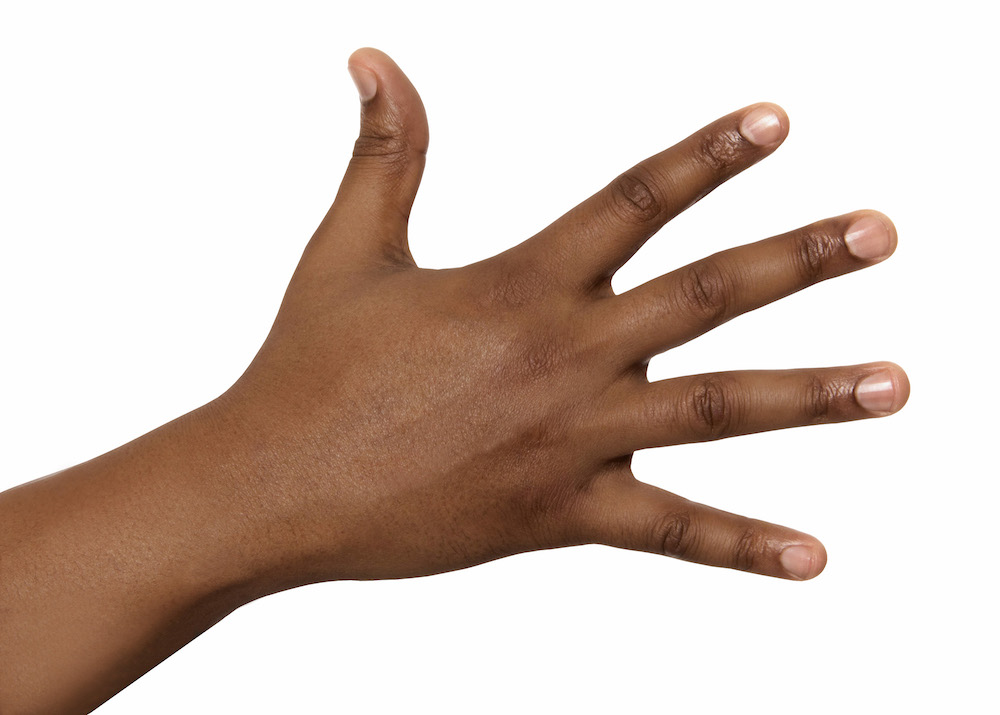
\includegraphics[width=\textwidth,height=\textheight,keepaspectratio]{../inputs/hand_dark.jpg}
  \end{minipage} & 
  \begin{minipage}{.29\textwidth}
    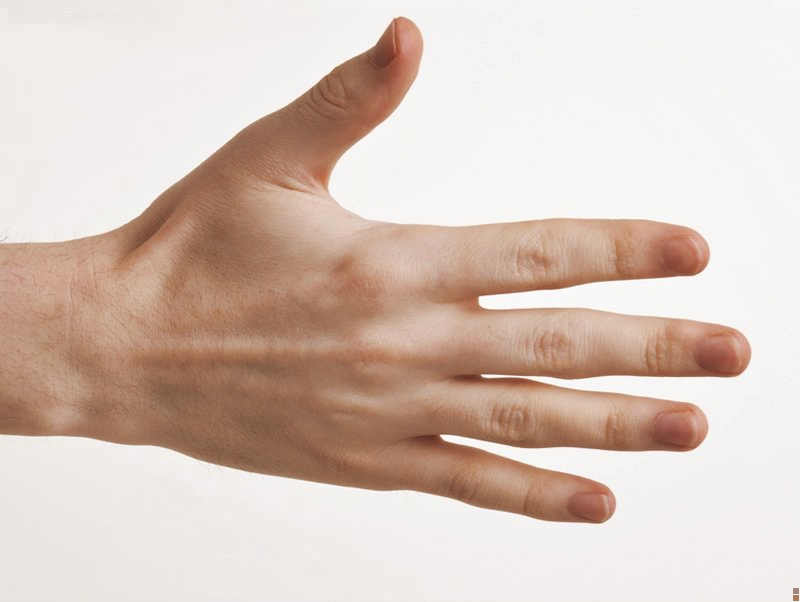
\includegraphics[width=\textwidth,height=\textheight,keepaspectratio]{../rc_test/outputs/20170524_prop_corr_1p1_ave_5/hand_pale_to_hand_dark.jpg}
  \end{minipage} \\
\hline
	  \ref{row:PY_NAME_hand_pale_to_hand_brown} &
  \begin{minipage}{.29\textwidth}
    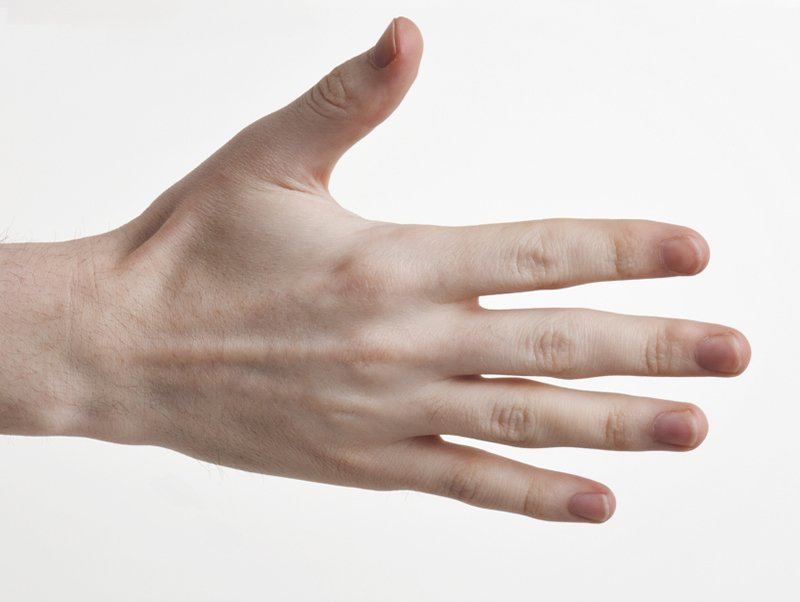
\includegraphics[width=\textwidth,height=\textheight,keepaspectratio]{../inputs/hand_pale.jpg}
  \end{minipage} & 
  \begin{minipage}{.29\textwidth}
    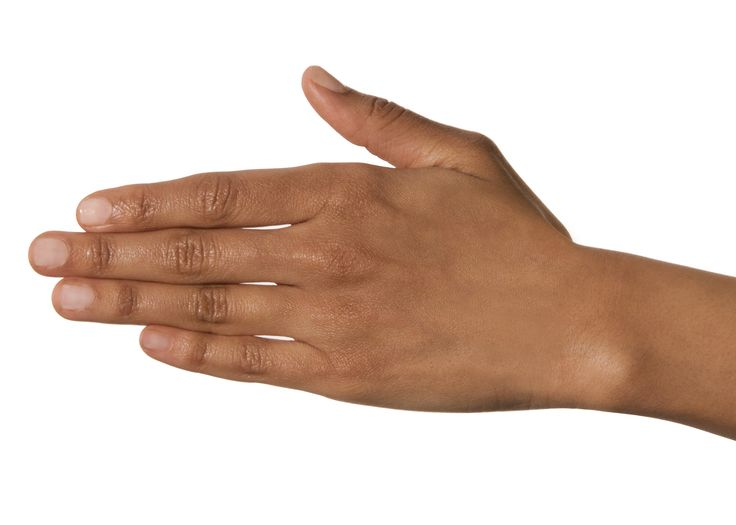
\includegraphics[width=\textwidth,height=\textheight,keepaspectratio]{../inputs/hand_brown.jpg}
  \end{minipage} & 
  \begin{minipage}{.29\textwidth}
    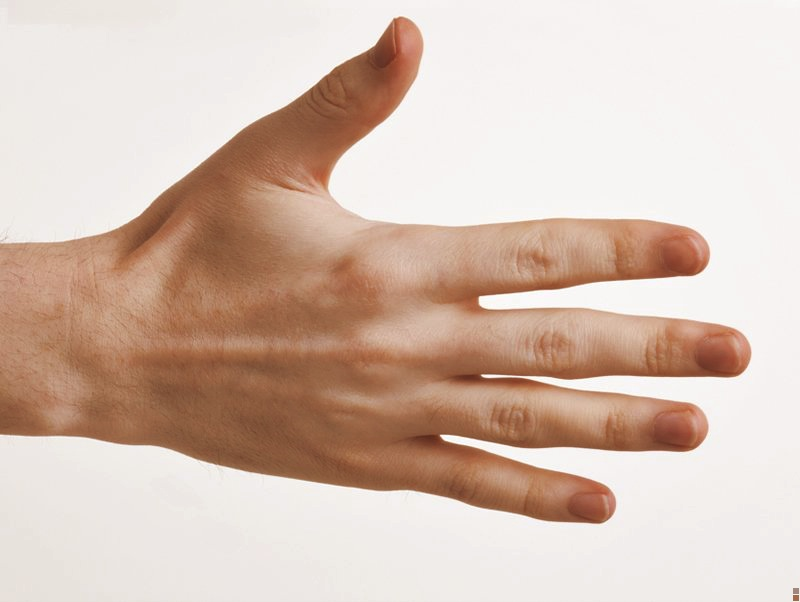
\includegraphics[width=\textwidth,height=\textheight,keepaspectratio]{../rc_test/outputs/20170524_prop_corr_1p1_ave_100/hand_pale_to_hand_brown.jpg}
  \end{minipage} \\
\hline
	  \ref{row:PY_NAME_hand_pale_to_hand_light} &
  \begin{minipage}{.29\textwidth}
    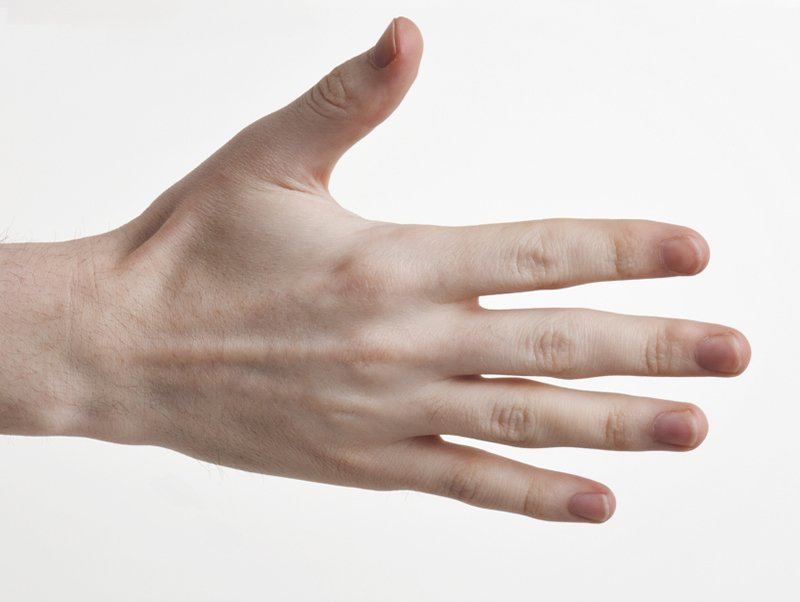
\includegraphics[width=\textwidth,height=\textheight,keepaspectratio]{../inputs/hand_pale.jpg}
  \end{minipage} & 
  \begin{minipage}{.29\textwidth}
    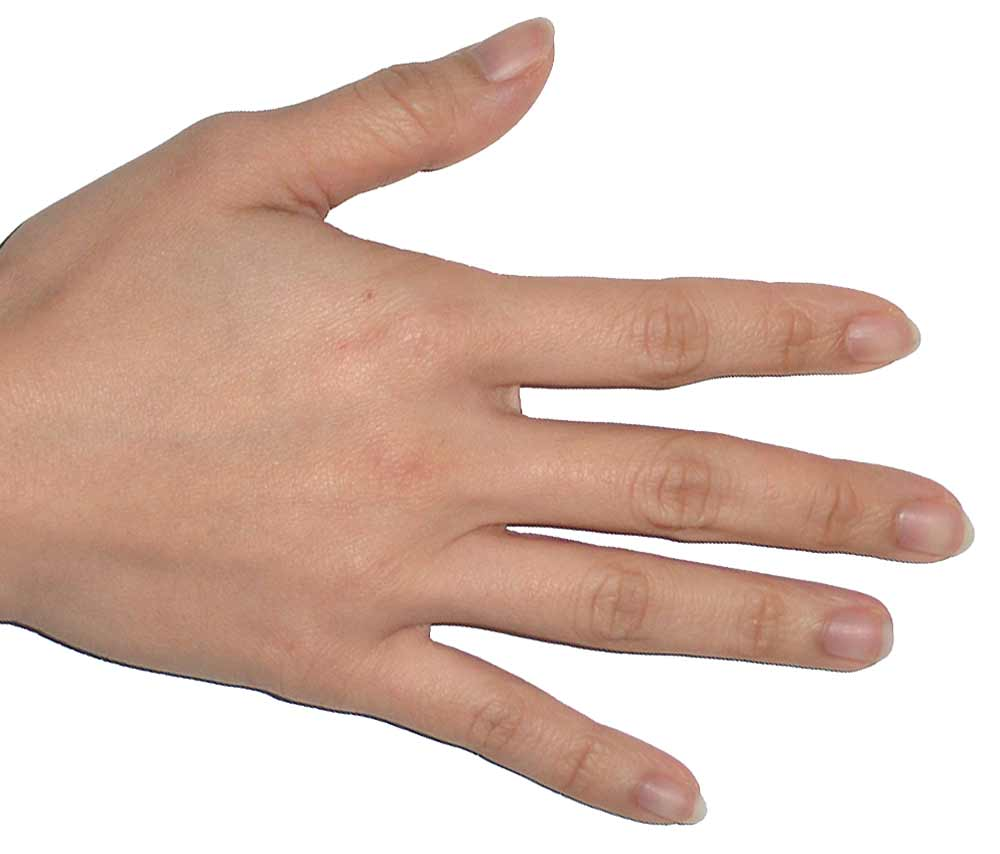
\includegraphics[width=\textwidth,height=\textheight,keepaspectratio]{../inputs/hand_light.jpg}
  \end{minipage} & 
  \begin{minipage}{.29\textwidth}
    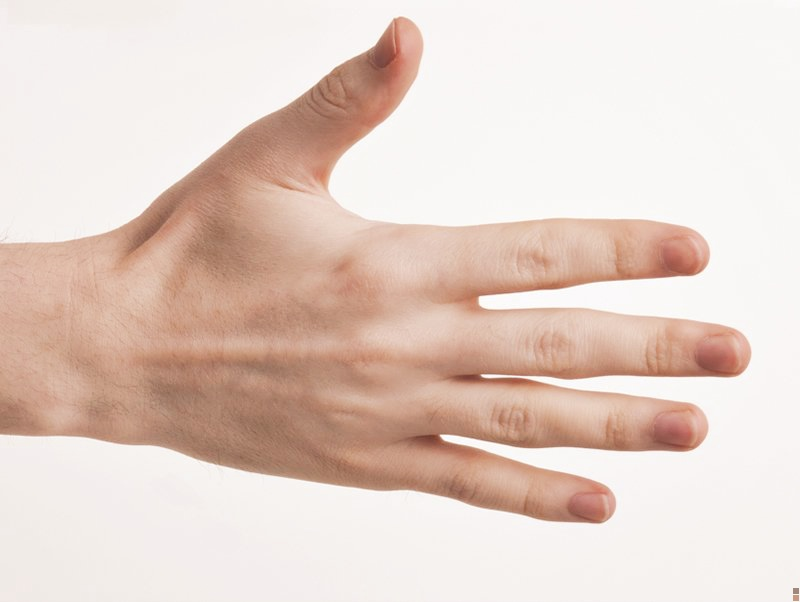
\includegraphics[width=\textwidth,height=\textheight,keepaspectratio]{../rc_test/outputs/20170524_prop_corr_1p1_ave_100/hand_pale_to_hand_light.jpg}
  \end{minipage} \\
\hline

 \end{longtable}

% \subsubsection*{Evaluation}
% As shown in Figure \ref{img:compare_dark_spot}, the dark spots and creases noted in Section \ref{sec:algo_prop_eval} are reduced.

% \begin{figure}[H]
%     \centering
%     \begin{subfigure}[b]{0.40\textwidth}
%         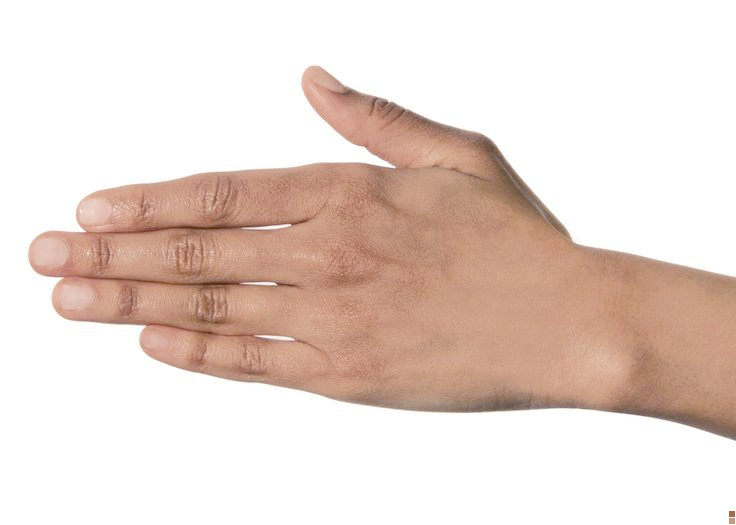
\includegraphics[width=\textwidth]{../rc_test/outputs/20170516_proportional_test/hand_brown_to_hand_light.jpg}
%         \caption{Proportional adjustment algorithm (Equation \ref{eq:prop_algo})result}
%     \end{subfigure}
%     ~
%     \begin{subfigure}[b]{0.40\textwidth}
%         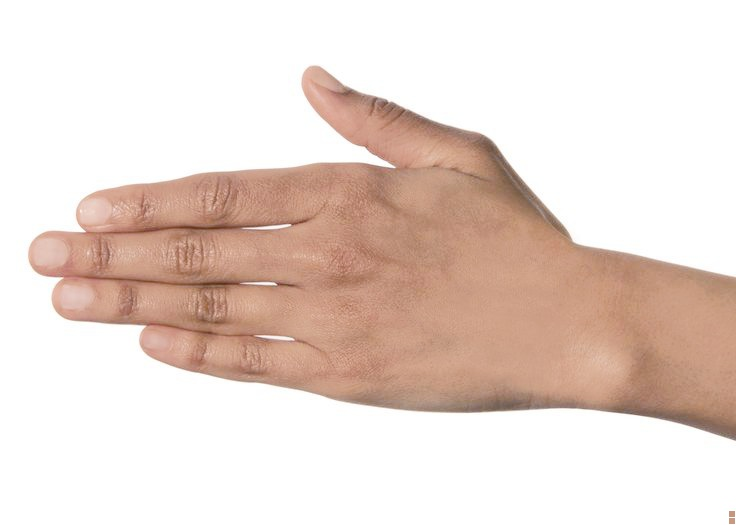
\includegraphics[width=\textwidth]{../rc_test/outputs/20170522_proportional_corrected_test_alpha1p1/hand_brown_to_hand_light.jpg}
%         \caption{Proportional adjustment algorithm with correction (Equation \ref{eq:prop_corr_algo}) result}
%     \end{subfigure}
%     \caption{Comparison of algorithms \ref{eq:prop_algo} and \ref{eq:prop_corr_algo} results for transforming a mid-toned hand (Figure \ref{img:input_hands_1_brown}) to a light hand (Figure \ref{img:input_hands_1_light}).\label{img:compare_dark_spot}}
% \end{figure}

% We tried this effect for a range of $\alpha$ and found that $\alpha = 1.1$ gives an acceptably realistic result. A larger $\alpha$ would further reduce the dark spots on the skin but may begin to strongly brighten the shadows of the image, resulting in an unrealistic effect.

% Up to the current iteration the more extreme changes of luminosity, such as from Figure \ref{img:input_hands_1_dark} to Figure \ref{img:input_hands_1_pale} and vice versa are especially unrealistic. Part of the reason is that the shadows, most prominent in Figure \ref{img:input_hands_1_pale} may be causing the average colour of the entire hand to be of lower luminosity than it should be. 